\documentclass[gr-notes.tex]{subfiles}

\begin{document}

\setcounter{chapter}{7}

\chapter{The Einstein field equations}

\setcounter{section}{5}

\section{Exercises}

\textbf{3}

(a) Calculate in geometrized units:

(i) the Newtonian potential of the Sun at its surface
%
\begin{displaymath}
  \phi =
 -G M_\Sun / R_\Sun \approx
 -\SI{1.476e3}{m} / \SI{6.960e8}{m} \approx
  \num{-2.12e-6}
\end{displaymath}

(ii) the Newtonian potential of the Sun at the radius of Earth's orbit
%
\begin{displaymath}
  \phi =
 -G M_\Sun / \SI{1}{AU} \approx
 -\SI{1.476e3}{m} / \SI{1.496e11}{m} \approx
  \num{-9.866e-9}
\end{displaymath}

(iii) the Newtonian potential of the Earth at its surface
%
\begin{displaymath}
  \phi =
 -G M_\Earth / R_\Earth \approx
 -\SI{4.434e-3}{m} / \SI{6.371e6}{m} \approx
  \num{-9.660e-10}
\end{displaymath}

(iv) the Earth's orbital velocity

Here I use the result from part (c), and find that
%
\begin{displaymath}
  v =
  \sqrt{-\phi} \approx
  \num{9.933e-5}
\end{displaymath}

(b) If the potential due to the Sun at Earth's orbital radius is greater than the Earth's potential at its surface (as is shown above), then why do we feel the Earth's gravity more than the Sun's?

We don't feel the potential directly, we feel the gravitational acceleration it produces. Acceleration is obtained from the potential via $\vb{a} = -\grad\phi$, and in the case of a circular orbit in a Newtonian potential:
%
\begin{displaymath}
  a =
 -\grad\phi =
 -\pdv{r} (-G M / r) =
 -G m / r^2 =
  \phi / r.
\end{displaymath}
%
So in the two cases mentioned, we need to divide by the radius once more, to obtain the acceleration.
%
\begin{align*}
  a_\Sun &=
  \phi_\Sun / \SI{1}{AU} \approx
  \SI{-6.595e-20}{\per\meter}
  \\
  a_\Earth &=
  \phi_\Earth / R_\Earth \approx
  \SI{-1.092e-16}{\per\meter}
\end{align*}
%
As you can see, the acceleration due to the Earth is greater by a factor of $10^4$.

(c) Show that a circular orbit in a Newtonian potential has an orbital velocity $v^2 = -\phi$.

We saw above that $a = \phi / r$, and we also know that centripetal acceleration is given by $a = -v^2 / r$. Equating the two we get $v^2 = -\phi$.


\textbf{8}

(a) Show that $\tensor{R}{^\alpha_{\beta\mu\nu}} = \eta^{\alpha\sigma} R_{\alpha\beta\mu\nu} + \order*{[h_{\alpha\beta}]^2}$.

\begin{align*}
  \tensor{R}{^\alpha_{\beta\mu\nu}} &=
  g^{\alpha\sigma} R_{\sigma\beta\mu\nu} =
  (\eta^{\alpha\sigma} + h^{\alpha\sigma}) R_{\sigma\beta\mu\nu} =
  \eta^{\alpha\sigma} R_{\sigma\beta\mu\nu} + h^{\alpha\sigma} R_{\sigma\beta\mu\nu}
  \\
  h^{\alpha\sigma} R_{\sigma\beta\mu\nu} &=
  \frac{1}{2} h^{\alpha\sigma}
  (h_{\sigma\nu,\beta\mu} + h_{\beta\mu,\sigma\nu} -
   h_{\sigma\mu,\beta\nu} - h_{\beta\nu,\sigma\mu}) =
  \order*{[h_{\alpha\beta}]^2}
\end{align*}

(b) Find $R_{\alpha\beta}$ to first order in $h_{\mu\nu}$.

\begin{align*}
  \tensor{R}{^\alpha_{\beta\mu\nu}} &\approx
  \eta^{\alpha\sigma} R_{\sigma\beta\mu\nu}
  \\
  \tensor{\delta}{^\mu_\alpha} \tensor{R}{^\alpha_{\beta\mu\nu}} &\approx
  R_{\beta\nu} \approx
  \tensor{\delta}{^\mu_\alpha} \eta^{\alpha\sigma} R_{\sigma\beta\mu\nu} \approx
  \eta^{\mu\sigma} R_{\sigma\beta\mu\nu}
\end{align*}

(c) Show that $g_{\alpha\beta} R = \eta_{\alpha\beta} \eta^{\mu\nu} R_{\mu\nu} + \order*{[h_{\alpha\beta}]^2}$.

\begin{align*}
  R &=
  g^{\mu\nu} R_{\mu\nu} =
  (\eta^{\mu\nu} + h^{\mu\nu}) R_{\mu\nu} =
  \eta^{\mu\nu} R_{\mu\nu} + \eta^{\mu\gamma} \eta^{\nu\lambda} R_{\mu\nu} =
  \eta^{\mu\nu} R_{\mu\nu} + \order*{[h_{\alpha\beta}]^2}
  \\
  g_{\alpha\beta} R &=
  g_{\alpha\beta} \eta^{\mu\nu} R_{\mu\nu} + \order*{[h_{\alpha\beta}]^2} =
  (\eta_{\alpha\beta} + h_{\alpha\beta})
  \eta^{\mu\nu} R_{\mu\nu} + \order*{[h_{\alpha\beta}]^2} =
  \eta_{\alpha\beta} \eta^{\mu\nu} R_{\mu\nu} + \order*{[h_{\alpha\beta}]^2}
\end{align*}

(d) Use this to show that $G_{\alpha\beta} = R_{\alpha\beta} - \frac{1}{2} \eta_{\alpha\beta} R$.

\begin{displaymath}
  G_{\alpha\beta} =
  R_{\alpha\beta} - \frac{1}{2} g_{\alpha\beta} R =
  R_{\alpha\beta} - \frac{1}{2} (\eta_{\alpha\beta} \eta^{\mu\nu} R_{\mu\nu}) =
  R_{\alpha\beta} - \frac{1}{2} \eta_{\alpha\beta} R
\end{displaymath}

(e) Now use this to simplify the calculation of Equation 8.32.

I got stuck here. I began by expanding the expression in (d) using the results from previous sections, shown in Figure \ref{fig:ch8-problem8e-i}. Then I expanded Equation 8.32, to get it in a more similar form, in Figures \ref{fig:ch8-problem8e-ii} and \ref{fig:ch8-problem8e-iii}. I did this with the hope of matching terms in the two equations, but was only able to match one. I believe something that would help me get further is Equation 8.33, $\tensor{\bar{h}}{^{\mu\nu}_{,\nu}} = 0$.

\begin{figure}[ht]
  \centering
  \begin{subfigure}[b]{0.8\textwidth}
    \includegraphics[width=\textwidth]{img/ch8_problem_8e_part3}
    \caption{}
    \label{fig:ch8-problem8e-i}
  \end{subfigure}

  \begin{subfigure}[b]{0.5\textwidth}
    \includegraphics[width=\textwidth]{img/ch8_problem_8e_part1}
    \caption{}
    \label{fig:ch8-problem8e-ii}
  \end{subfigure}
  ~
  \begin{subfigure}[b]{0.3\textwidth}
    \includegraphics[width=\textwidth]{img/ch8_problem_8e_part2}
    \caption{}
    \label{fig:ch8-problem8e-iii}
  \end{subfigure}
  \caption{Incomplete solution to Problem 8.8 (e)}
\end{figure}


\textbf{9}

(a)

% I start this by making a simplification on Equation 8.32, by using Equation 8.33. In 8.32 we have the term $\tensor{\bar{h}}{_{\mu\nu}^{,\mu\nu}}$. If we can get this into the form of 8.33, we can cancel it out. This is easy to show
% %
% \begin{displaymath}
%   \tensor{\bar{h}}{_{\mu\nu}^{,\mu\nu}} =
%   \eta^{\mu\alpha} \eta^{\nu\beta} \tensor{\bar{h}}{_{\mu\nu,\mu\nu}} =
%   \tensor{\bar{h}}{^{\alpha\beta}_{,\alpha\beta}} = 0.
% \end{displaymath}
% %
% So Equation 8.32 then becomes
% %
% \begin{displaymath}
%   G_{\alpha\beta} =
%  -\frac{1}{2} [
%     \tensor{\bar{h}}{_{\alpha\beta,\mu}^{,\mu}} -
%     \tensor{\bar{h}}{_{\alpha\mu,\beta}^{,\mu}} -
%     \tensor{\bar{h}}{_{\beta\mu,\alpha}^{,\mu}} +
%     \order*{[h_{\alpha\beta}]^2}
%   ]
% \end{displaymath}

I start by making a slight rewrite of Equation 8.32, changing the second $\bar{h}$ term.
%
\begin{displaymath}
  \eta_{\alpha\beta} \tensor{\bar{h}}{_{\mu\nu}^{,\mu\nu}} =
  \eta_{\alpha\beta} \eta^{\mu\alpha} \tensor{\bar{h}}{_{\mu\nu,\alpha}^{,\nu}} =
  \tensor{\bar{h}}{_{\beta\nu,\alpha}^{,\nu}}
\end{displaymath}
%
So now the Einstein tensor can be written as
%
\begin{displaymath}
  G_{\alpha\beta} =
 -\frac{1}{2} [
    \tensor{\bar{h}}{_{\alpha\beta,\mu}^{,\mu}} +
    \tensor{\bar{h}}{_{\beta\nu,\alpha}^{,\nu}} -
    \tensor{\bar{h}}{_{\alpha\mu,\beta}^{,\mu}} -
    \tensor{\bar{h}}{_{\beta\mu,\alpha}^{,\mu}} +
    \order*{[h_{\alpha\beta}]^2}
  ].
\end{displaymath}
%
For $G_{00}$ we then have
%
\begin{align*}
  G_{00} &=
 -\frac{1}{2} [
    \tensor{\bar{h}}{_{00,\mu}^{,\mu}} +
    \tensor{\bar{h}}{_{0\nu,0}^{,\nu}} -
    \tensor{\bar{h}}{_{0\mu,0}^{,\mu}} -
    \tensor{\bar{h}}{_{0\mu,0}^{,\mu}} +
    \order*{[h_{00}]^2}
  ]
  \\ &=
 -\frac{1}{2} [
    \tensor{\bar{h}}{_{00,\mu}^{,\mu}} -
    \tensor{\bar{h}}{_{0\mu,0}^{,\mu}} +
    \order*{[h_{00}]^2}
  ]
  \\ &=
 -\frac{1}{2} [
    (\tensor{\bar{h}}{_{00,0}^{,0}} + \tensor{\bar{h}}{_{00,i}^{,i}}) -
    (\tensor{\bar{h}}{_{00,0}^{,0}} + \tensor{\bar{h}}{_{0i,0}^{,i}}) +
    \order*{[h_{00}]^2}
  ]
  \\ &=
 -\frac{1}{2} [
    \tensor{\bar{h}}{_{00,i}^{,i}} -
    \tensor{\bar{h}}{_{0i,0}^{,i}} +
    \order*{[h_{00}]^2}
  ],
\end{align*}
%
which contains no second time derivatives. For $G_{0i}$ I encountered a problem:
%
\begin{align*}
  G_{0i} &=
 -\frac{1}{2} [
    \tensor{\bar{h}}{_{0i,\mu}^{,\mu}} +
    \tensor{\bar{h}}{_{i\nu,0}^{,\nu}} -
    \tensor{\bar{h}}{_{0\mu,i}^{,\mu}} -
    \tensor{\bar{h}}{_{i\mu,0}^{,\mu}} +
    \order*{[h_{0i}]^2}
  ]
  \\ &=
 -\frac{1}{2} [
    \tensor{\bar{h}}{_{0i,\mu}^{,\mu}} -
    \tensor{\bar{h}}{_{0\mu,i}^{,\mu}} +
    \order*{[h_{0i}]^2}
  ]
  \\ &=
 -\frac{1}{2} [
    (\tensor{\bar{h}}{_{0i,0}^{,0}} + \tensor{\bar{h}}{_{0i,j}^{,j}}) -
    \tensor{\bar{h}}{_{0\mu,i}^{,\mu}} +
    \order*{[h_{0i}]^2}
  ],
\end{align*}
%
which retains a second time derivative in the $\tensor{\bar{h}}{_{0i,0}^{,0}}$ term.

(b)

According to Schutz's solution it is not a contradiction, due in part to Equation 8.33. I don't fully understand the reason, though.


\textbf{11}
Write the gauge transformation and Lorentz gauge condition in four-tensor notation for Maxwell's equations. Draw an analogy with linearized gravity.

First we rewrite $\phi \to \phi - \pdv*{f}{t}$ as $-A_0 \to -A_0 - f_{,0}$, and cancelling the negatives we get $A_0 \to A_0 + f_{,0}$. Combining this with $A_i \to A_i + f_{,i}$, it is obvious that the gauge transformation generalizes to $A_\alpha \to A_\alpha + f_{,\alpha}$.

The Lorentz gauge condition is just slightly less obvious. We start by noting that $A_0 = -\phi$, and therefore (in Minkowski space) $A^0 = \eta^{0\mu} A_\mu = g^{00} A_0 = (-1) (-\phi) = \phi$. Then the Lorentz gauge condition  becomes $\tensor{A}{^0_{,0}} + \tensor{A}{^i_{,i}} = \tensor{A}{^\alpha_{,\alpha}} = 0$.



\textbf{13}
Give a physical justification for $\abs{T^{00}} \gg \abs{T^{0i}} \gg \abs{T^{ij}}$ in a Newtonian system.

The first inequality is easy to see. $T^{00} = E / V = p^0 / V$, and $T^{0i} = p^i / V$. In the Newtonian limit, $\abs{p^0} \gg \abs{p^i}$, and so it follows that $\abs{T^{00}} \gg \abs{T^{0i}}$.

The second inequality is less obvious. In the Newtonian limit, forces must be relatively small, or else objects would be accelerated to relativistic speeds. By this argument, the stresses must also be relatively small, and so $T^{0i} \gg T^{ij}$.

\textbf{17}

(a) First I need to convert the orbital period into meters.
%
\begin{displaymath}
  T =
  \SI{200}{days} \times
  \frac{\SI{24}{hours}}{\SI{1}{day}} \times
  \frac{\SI{3600}{seconds}}{\SI{1}{hour}} \times
  c \approx
  \SI{5.18e15}{\meter}
\end{displaymath}
%
Then I use the potential to find the speed, which I relate to the circumference and orbital period, and solve for the mass.
%
\begin{gather*}
  \phi = -G M / r
  \\
  v^2 = -\phi
\end{gather*}
\begin{align*}
  M &= v^2 r / G = C^3 / (2 \pi T^2 G) \approx
  (\SI{6e11}{\meter})^3 / (2 \pi (\SI{5.18e15}{\meter})^2 G)
  \\ &\approx
  \SI{1.281e3}{\meter} \times \frac{1 M_\Sun}{\SI{1.476e3}{m}} \approx
  0.868 M_\Sun
\end{align*}

(b)

Using the above formula, I get a distribution of mass estimates, shown in Figure \ref{fig:ch8-problem17b}. Closer to the black hole, the Newtonian approximation breaks down, and the ``effective mass'' blows up. Far from the black hole, we can see that the effective mass is in agreement for all of the sattelites, and so the Newtonian approximation is working again. Thus, I use the furthest sattelite to find that the black hole's mass is $68 M_\Sun$.

\begin{figure}[ht]
  \centering
  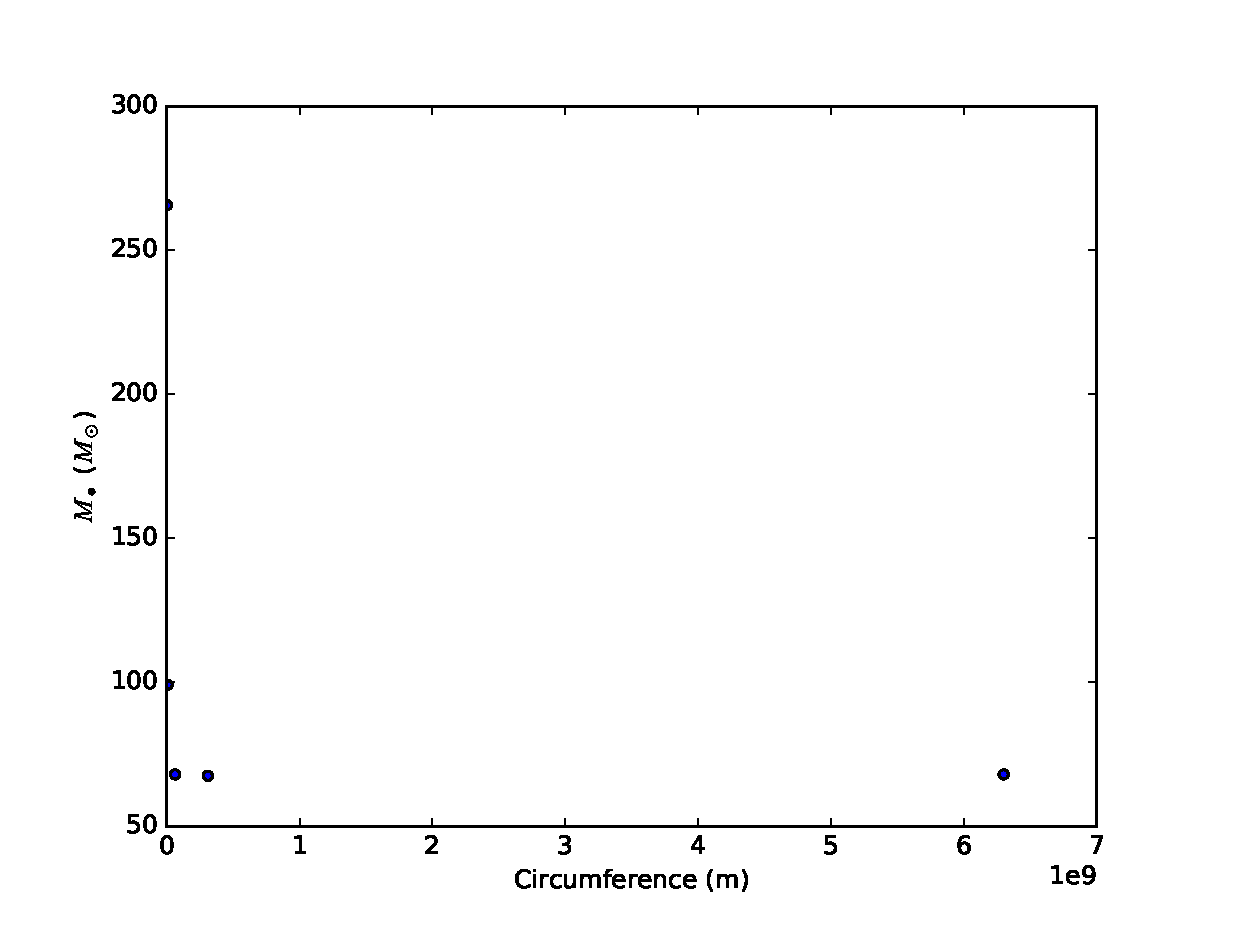
\includegraphics[width=0.6\textwidth]{img/ch8_problem_17b}
  \caption{Black hole mass estimates in Problem 8.17, as a function of sattelite circumference.}
  \label{fig:ch8-problem17b}
\end{figure}



\end{document}